\documentclass[12pt,a4paper]{article}
\usepackage[utf8]{inputenc}
\usepackage[english]{babel}
\usepackage[T1]{fontenc}
\usepackage{amsmath}
\usepackage{amsfonts}
\usepackage{amssymb}
\usepackage{makeidx}
\usepackage{graphicx}
\usepackage{kpfonts}
\usepackage[left=3cm,right=2cm,top=3cm,bottom=3cm]{geometry}
\usepackage{float}
\usepackage{adjustbox}
\usepackage{booktabs}
\usepackage{multirow}
\newcommand\x{\times}
\begin{document}
In this tests are considered 4 types of combinations:
\begin{itemize}
\item $c1$
\begin{center}
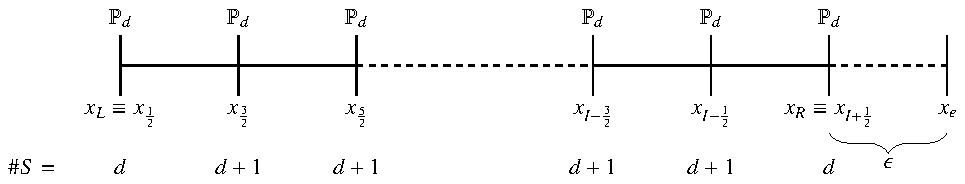
\includegraphics[width=.75\textwidth]{images/c1.pdf}
\end{center}
\item $c2$
\begin{center}
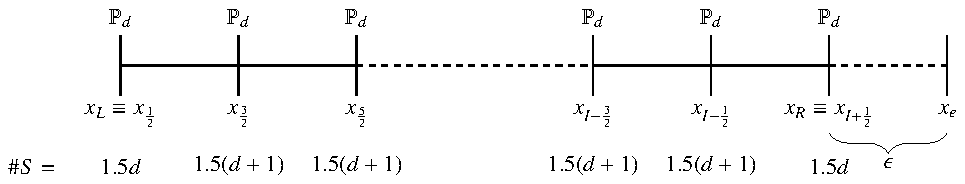
\includegraphics[width=.75\textwidth]{images/c2.pdf}
\end{center}
\item $c3$
\begin{center}
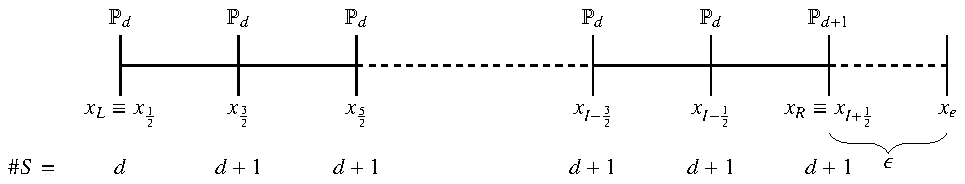
\includegraphics[width=.75\textwidth]{images/c3.pdf}
\end{center}
\item $c4$
\begin{center}
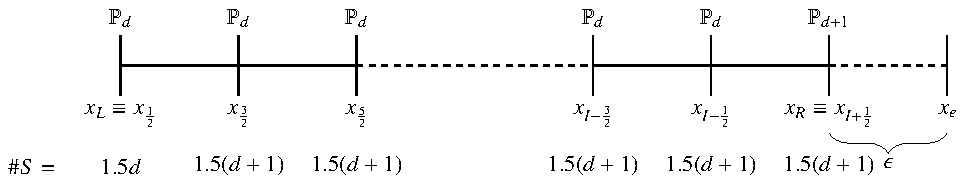
\includegraphics[width=.75\textwidth]{images/c4.pdf}
\end{center}
\end{itemize}
\pagebreak
\section*{$\epsilon=0$ -- uniform mesh}
\begin{table}[H]
\centering
\caption{Numerical results of pure diffusion for $\phi(x)=\exp(x)$, $\kappa(x)=1$, and $u(x)=0+$ (c1; uniform mesh; $\epsilon=0$).}
\begin{tabular}{@{}l c c c l c c l c c l c c@{}}
\toprule
 & $I$ & cond(A) & $A^{-1}\geq 0$ &  E$_{c,1}$ & O$_{c,1}$ && E$_1$ & O$_1$ && E$_{\infty}$ & O$_{\infty}$\\
\midrule
\multirow{3}{*}{$\mathbb{P}_{1}$}
 & 20 & 6.48E$+$02 & $\checkmark$ & 8.76E$-$04 & --- && 5.66E$-$04 & --- && 7.61E$-$04 & ---\\
 & 40 & 2.59E$+$03 & $\checkmark$ & 2.14E$-$04 & 2.03 && 1.42E$-$04 & 2.00 && 1.92E$-$04 & 1.99\\
 & 80 & 1.04E$+$04 & $\checkmark$ & 5.28E$-$05 & 2.02 && 3.54E$-$05 & 2.00 && 4.82E$-$05 & 1.99\\
\midrule
\multirow{3}{*}{$\mathbb{P}_{2}$}
 & 20 & 8.25E$+$02 & $\checkmark$ & 7.53E$-$05 & --- && 1.40E$-$04 & --- && 3.33E$-$04 & ---\\
 & 40 & 3.30E$+$03 & $\checkmark$ & 9.55E$-$06 & 2.98 && 3.61E$-$05 & 1.95 && 8.64E$-$05 & 1.95\\
 & 80 & 1.32E$+$04 & $\checkmark$ & 1.20E$-$06 & 2.99 && 9.19E$-$06 & 1.97 && 2.20E$-$05 & 1.97\\
\midrule
\multirow{3}{*}{$\mathbb{P}_{3}$}
 & 20 & 1.02E$+$03 & $\checkmark$ & 4.41E$-$06 & --- && 6.53E$-$07 & --- && 7.67E$-$07 & ---\\
 & 40 & 4.08E$+$03 & $\checkmark$ & 2.78E$-$07 & 3.99 && 4.07E$-$08 & 4.01 && 5.30E$-$08 & 3.86\\
 & 80 & 1.63E$+$04 & $\checkmark$ & 1.75E$-$08 & 3.99 && 2.53E$-$09 & 4.01 && 3.47E$-$09 & 3.93\\
\midrule
\multirow{3}{*}{$\mathbb{P}_{4}$}
 & 20 & 1.18E$+$03 & $\checkmark$ & 2.00E$-$07 & --- && 2.39E$-$08 & --- && 5.60E$-$08 & ---\\
 & 40 & 4.74E$+$03 & $\checkmark$ & 6.36E$-$09 & 4.98 && 2.07E$-$09 & 3.53 && 5.53E$-$09 & 3.34\\
 & 80 & 1.89E$+$04 & $\checkmark$ & 2.01E$-$10 & 4.99 && 1.59E$-$10 & 3.70 && 4.07E$-$10 & 3.77\\
\midrule
\multirow{3}{*}{$\mathbb{P}_{5}$}
 & 20 & 1.35E$+$03 & $\checkmark$ & 8.78E$-$09 & --- && 1.80E$-$09 & --- && 2.09E$-$09 & ---\\
 & 40 & 5.42E$+$03 & $\checkmark$ & 1.40E$-$10 & 5.97 && 2.70E$-$11 & 6.06 && 3.07E$-$11 & 6.09\\
 & 80 & 2.17E$+$04 & $\checkmark$ & 2.24E$-$12 & 5.96 && 1.53E$-$13 & 7.47 && 8.86E$-$13 & 5.11\\
\bottomrule
\end{tabular}
\end{table}
\begin{table}[H]
\centering
\caption{Numerical results of pure diffusion for $\phi(x)=\exp(x)$, $\kappa(x)=1$, and $u(x)=0$ (c2; uniform mesh; $\epsilon=0$).}
\begin{tabular}{@{}l c c c l c c l c c l c c@{}}
\toprule
 & $I$ & cond(A) & $A^{-1}\geq 0$ &  E$_{c,1}$ & O$_{c,1}$ && E$_1$ & O$_1$ && E$_{\infty}$ & O$_{\infty}$\\
\midrule
\multirow{2}{*}{$\mathbb{P}_{1}$}
 & 10 & 1.54E$+$02 & $\x$ & 8.54E$-$02 & --- && 7.55E$-$01 & --- && 1.85E$+$00 & ---\\
 & 20 & 1.51E$+$05 & $\x$ & 2.28E$-$02 & 1.90 && 1.70E$+$02 & $\uparrow$ && 5.08E$+$02 & $\uparrow$\\
\midrule
\multirow{2}{*}{$\mathbb{P}_{2}$}
 & 10 & 9.76E$+$01 & $\x$ & 6.48E$-$03 & --- && 5.01E$-$03 & --- && 1.10E$-$02 & ---\\
 & 20 & 3.86E$+$02 & $\checkmark$ & 9.18E$-$04 & 2.82 && 1.30E$-$03 & 1.94 && 3.22E$-$03 & 1.77\\
\midrule
\multirow{2}{*}{$\mathbb{P}_{3}$}
 & 10 & 1.29E$+$02 & $\checkmark$ & 3.02E$-$04 & --- && 3.15E$-$05 & --- && 7.63E$-$05 & ---\\
 & 20 & 5.17E$+$02 & $\checkmark$ & 1.86E$-$05 & 4.02 && 1.54E$-$06 & 4.36 && 5.01E$-$06 & 3.93\\
\midrule
\multirow{2}{*}{$\mathbb{P}_{4}$}
 & 10 & 1.88E$+$02 & $\checkmark$ & 3.54E$-$05 & --- && 4.08E$-$06 & --- && 9.67E$-$06 & ---\\
 & 20 & 7.50E$+$02 & $\checkmark$ & 1.19E$-$06 & 4.90 && 7.72E$-$07 & 2.40 && 1.84E$-$06 & 2.39\\
\midrule
\multirow{2}{*}{$\mathbb{P}_{5}$}
 & 10 & 2.00E$+$02 & $\checkmark$ & 5.69E$-$06 & --- && 7.61E$-$07 & --- && 1.43E$-$06 & ---\\
 & 20 & 7.98E$+$02 & $\checkmark$ & 8.96E$-$08 & 5.99 && 6.61E$-$09 & 6.85 && 2.08E$-$08 & 6.10\\
\bottomrule
\end{tabular}
\end{table}

%%%%%
\section*{$\epsilon=\frac{h^2}{2}$ -- uniform mesh}
\begin{table}[H]
\centering
\caption{Numerical results of pure diffusion for $\phi(x)=\exp(x)$, $\kappa(x)=1$, and $u(x)=0+$ (c1; uniform mesh; $\epsilon=\frac{h^2}{2}$).}
\begin{tabular}{@{}l c c c l c c l c c l c c@{}}
\toprule
 & $I$ & cond(A) & $A^{-1}\geq 0$ &  E$_{c,1}$ & O$_{c,1}$ && E$_1$ & O$_1$ && E$_{\infty}$ & O$_{\infty}$\\
\midrule
\multirow{3}{*}{$\mathbb{P}_{1}$}
 & 20 & 6.48E$+$02 & $\checkmark$ & 9.92E$-$04 & --- && 1.19E$-$03 & --- && 2.55E$-$03 & ---\\
 & 40 & 2.59E$+$03 & $\checkmark$ & 2.28E$-$04 & 2.12 && 2.97E$-$04 & 2.00 && 6.47E$-$04 & 1.98\\
 & 80 & 1.04E$+$04 & $\checkmark$ & 5.46E$-$05 & 2.06 && 7.42E$-$05 & 2.00 && 1.63E$-$04 & 1.99\\
\midrule
\multirow{3}{*}{$\mathbb{P}_{2}$}
 & 20 & 8.27E$+$02 & $\checkmark$ & 7.05E$-$05 & --- && 9.70E$-$05 & --- && 2.50E$-$04 & ---\\
 & 40 & 3.30E$+$03 & $\checkmark$ & 9.24E$-$06 & 2.93 && 3.08E$-$05 & 1.65 && 7.59E$-$05 & 1.72\\
 & 80 & 1.32E$+$04 & $\checkmark$ & 1.18E$-$06 & 2.97 && 8.53E$-$06 & 1.85 && 2.07E$-$05 & 1.88\\
\midrule
\multirow{3}{*}{$\mathbb{P}_{3}$}
 & 20 & 1.02E$+$03 & $\checkmark$ & 4.25E$-$06 & --- && 1.41E$-$06 & --- && 2.19E$-$06 & ---\\
 & 40 & 4.08E$+$03 & $\checkmark$ & 2.73E$-$07 & 3.96 && 8.88E$-$08 & 3.99 && 1.40E$-$07 & 3.97\\
 & 80 & 1.63E$+$04 & $\checkmark$ & 1.73E$-$08 & 3.98 && 5.58E$-$09 & 3.99 && 8.85E$-$09 & 3.99\\
\midrule
\multirow{3}{*}{$\mathbb{P}_{4}$}
 & 20 & 1.19E$+$03 & $\checkmark$ & 1.95E$-$07 & --- && 2.28E$-$08 & --- && 4.92E$-$08 & ---\\
 & 40 & 4.74E$+$03 & $\checkmark$ & 6.27E$-$09 & 4.96 && 1.92E$-$09 & 3.57 && 5.18E$-$09 & 3.25\\
 & 80 & 1.90E$+$04 & $\checkmark$ & 1.99E$-$10 & 4.98 && 1.53E$-$10 & 3.65 && 3.94E$-$10 & 3.72\\
\midrule
\multirow{3}{*}{$\mathbb{P}_{5}$}
 & 20 & 1.36E$+$03 & $\checkmark$ & 8.57E$-$09 & --- && 1.07E$-$09 & --- && 4.89E$-$09 & ---\\
 & 40 & 5.42E$+$03 & $\checkmark$ & 1.38E$-$10 & 5.96 && 1.84E$-$11 & 5.86 && 8.81E$-$11 & 5.79\\
 & 80 & 2.17E$+$04 & $\checkmark$ & 2.22E$-$12 & 5.95 && 5.11E$-$13 & 5.17 && 1.87E$-$12 & 5.56\\
\bottomrule
\end{tabular}
\end{table}
\begin{table}[H]
\centering
\caption{Numerical results of pure diffusion for $\phi(x)=\exp(x)$, $\kappa(x)=1$, and $u(x)=0$ (c2; uniform mesh; $\epsilon=\frac{h^2}{2}$).}
\begin{tabular}{@{}l c c c l c c l c c l c c@{}}
\toprule
 & $I$ & cond(A) & $A^{-1}\geq 0$ &  E$_{c,1}$ & O$_{c,1}$ && E$_1$ & O$_1$ && E$_{\infty}$ & O$_{\infty}$\\
\midrule
\multirow{3}{*}{$\mathbb{P}_{1}$}
 & 20 & 4.68E$+$03 & $\x$ & 9.52E$-$03 & --- && 8.66E$-$01 & --- && 5.82E$+$00 & ---\\
 & 40 & 1.56E$+$07 & $\x$ & 2.41E$-$03 & 1.98 && 3.45E$+$02 & $\uparrow$ && 4.60E$+$03 & $\uparrow$\\
 & 80 & 1.71E$+$14 & $\x$ & 6.06E$-$04 & 1.99 && 4.68E$+$08 & $\uparrow$ && 1.25E$+$10 & $\uparrow$\\
\midrule
\multirow{3}{*}{$\mathbb{P}_{2}$}
 & 20 & 5.25E$+$02 & $\checkmark$ & 3.51E$-$04 & --- && 4.89E$-$04 & --- && 1.20E$-$03 & ---\\
 & 40 & 2.09E$+$03 & $\checkmark$ & 4.56E$-$05 & 2.94 && 1.41E$-$04 & 1.79 && 3.41E$-$04 & 1.81\\
 & 80 & 8.36E$+$03 & $\checkmark$ & 5.81E$-$06 & 2.97 && 3.77E$-$05 & 1.91 && 9.04E$-$05 & 1.91\\
\midrule
\multirow{3}{*}{$\mathbb{P}_{3}$}
 & 20 & 5.99E$+$02 & $\checkmark$ & 1.52E$-$05 & --- && 6.12E$-$06 & --- && 1.12E$-$05 & ---\\
 & 40 & 2.39E$+$03 & $\checkmark$ & 9.77E$-$07 & 3.96 && 4.35E$-$07 & 3.82 && 8.10E$-$07 & 3.79\\
 & 80 & 9.56E$+$03 & $\checkmark$ & 6.20E$-$08 & 3.98 && 3.14E$-$08 & 3.79 && 6.03E$-$08 & 3.75\\
\midrule
\multirow{3}{*}{$\mathbb{P}_{4}$}
 & 20 & 7.52E$+$02 & $\checkmark$ & 1.16E$-$06 & --- && 8.60E$-$07 & --- && 2.02E$-$06 & ---\\
 & 40 & 3.00E$+$03 & $\checkmark$ & 3.84E$-$08 & 4.92 && 6.80E$-$08 & 3.66 && 1.59E$-$07 & 3.66\\
 & 80 & 1.20E$+$04 & $\checkmark$ & 1.24E$-$09 & 4.96 && 4.65E$-$09 & 3.87 && 1.10E$-$08 & 3.86\\
\midrule
\multirow{3}{*}{$\mathbb{P}_{5}$}
 & 20 & 7.99E$+$02 & $\checkmark$ & 5.47E$-$08 & --- && 2.72E$-$08 & --- && 5.72E$-$08 & ---\\
 & 40 & 3.19E$+$03 & $\checkmark$ & 8.76E$-$10 & 5.96 && 7.88E$-$10 & 5.11 && 1.77E$-$09 & 5.01\\
 & 80 & 1.27E$+$04 & $\checkmark$ & 1.39E$-$11 & 5.98 && 2.35E$-$11 & 5.07 && 5.45E$-$11 & 5.03\\
\bottomrule
\end{tabular}
\end{table}
\begin{table}[H]
\centering
\caption{Numerical results of pure diffusion for $\phi(x)=\exp(x)$, $\kappa(x)=1$, and $u(x)=0$ (c3; uniform mesh; $\epsilon=\frac{h^2}{2}$).}
\begin{tabular}{@{}l c c c l c c l c c l c c@{}}
\toprule
 & $I$ & cond(A) & $A^{-1}\geq 0$ &  E$_{c,1}$ & O$_{c,1}$ && E$_1$ & O$_1$ && E$_{\infty}$ & O$_{\infty}$\\
\midrule
\multirow{3}{*}{$\mathbb{P}_{1}$}
 & 20 & 6.49E$+$02 & $\checkmark$ & 8.71E$-$04 & --- && 5.23E$-$04 & --- && 6.77E$-$04 & ---\\
 & 40 & 2.59E$+$03 & $\checkmark$ & 2.14E$-$04 & 2.03 && 1.36E$-$04 & 1.94 && 1.81E$-$04 & 1.90\\
 & 80 & 1.04E$+$04 & $\checkmark$ & 5.28E$-$05 & 2.02 && 3.47E$-$05 & 1.97 && 4.69E$-$05 & 1.95\\
\midrule
\multirow{3}{*}{$\mathbb{P}_{2}$}
 & 20 & 8.27E$+$02 & $\checkmark$ & 7.52E$-$05 & --- && 1.49E$-$04 & --- && 3.52E$-$04 & ---\\
 & 40 & 3.30E$+$03 & $\checkmark$ & 9.54E$-$06 & 2.98 && 3.75E$-$05 & 1.99 && 8.90E$-$05 & 1.98\\
 & 80 & 1.32E$+$04 & $\checkmark$ & 1.20E$-$06 & 2.99 && 9.36E$-$06 & 2.00 && 2.23E$-$05 & 2.00\\
\midrule
\multirow{3}{*}{$\mathbb{P}_{3}$}
 & 20 & 1.02E$+$03 & $\checkmark$ & 4.40E$-$06 & --- && 7.35E$-$07 & --- && 3.10E$-$06 & ---\\
 & 40 & 4.08E$+$03 & $\checkmark$ & 2.78E$-$07 & 3.98 && 4.87E$-$08 & 3.92 && 2.09E$-$07 & 3.89\\
 & 80 & 1.63E$+$04 & $\checkmark$ & 1.75E$-$08 & 3.99 && 3.13E$-$09 & 3.96 && 1.35E$-$08 & 3.95\\
\midrule
\multirow{3}{*}{$\mathbb{P}_{4}$}
 & 20 & 1.19E$+$03 & $\checkmark$ & 2.00E$-$07 & --- && 7.86E$-$08 & --- && 1.70E$-$07 & ---\\
 & 40 & 4.74E$+$03 & $\checkmark$ & 6.36E$-$09 & 4.97 && 9.83E$-$10 & 6.32 && 1.96E$-$09 & 6.43\\
 & 80 & 1.90E$+$04 & $\checkmark$ & 2.01E$-$10 & 4.99 && 7.92E$-$11 & 3.63 && 2.36E$-$10 & 3.05\\
\midrule
\multirow{3}{*}{$\mathbb{P}_{5}$}
 & 20 & 1.36E$+$03 & $\checkmark$ & 8.77E$-$09 & --- && 3.75E$-$09 & --- && 1.12E$-$08 & ---\\
 & 40 & 5.42E$+$03 & $\checkmark$ & 1.40E$-$10 & 5.97 && 6.42E$-$11 & 5.87 && 1.92E$-$10 & 5.87\\
 & 80 & 2.17E$+$04 & $\checkmark$ & 2.24E$-$12 & 5.96 && 1.32E$-$12 & 5.61 && 3.56E$-$12 & 5.75\\
\bottomrule
\end{tabular}
\end{table}
\begin{table}[H]
\centering
\caption{Numerical results of pure diffusion for $\phi(x)=\exp(x)$, $\kappa(x)=1$, and $u(x)=0$ (c4; uniform mesh; $\epsilon=\frac{h^2}{2}$).}
\begin{tabular}{@{}l c c c l c c l c c l c c@{}}
\toprule
 & $I$ & cond(A) & $A^{-1}\geq 0$ &  E$_{c,1}$ & O$_{c,1}$ && E$_1$ & O$_1$ && E$_{\infty}$ & O$_{\infty}$\\
\midrule
\multirow{3}{*}{$\mathbb{P}_{1}$}
 & 20 & 4.66E$+$03 & $\x$ & 9.36E$-$03 & --- && 8.64E$-$01 & --- && 5.74E$+$00 & ---\\
 & 40 & 1.55E$+$07 & $\x$ & 2.39E$-$03 & 1.97 && 3.58E$+$02 & $\uparrow$ && 4.54E$+$03 & $\uparrow$\\
 & 80 & 1.72E$+$14 & $\x$ & 6.03E$-$04 & 1.98 && 5.26E$+$08 & $\uparrow$ && 1.23E$+$10 & $\uparrow$\\
\midrule
\multirow{3}{*}{$\mathbb{P}_{2}$}
 & 20 & 5.25E$+$02 & $\checkmark$ & 3.44E$-$04 & --- && 5.59E$-$04 & --- && 1.33E$-$03 & ---\\
 & 40 & 2.09E$+$03 & $\checkmark$ & 4.51E$-$05 & 2.93 && 1.50E$-$04 & 1.89 && 3.58E$-$04 & 1.89\\
 & 80 & 8.36E$+$03 & $\checkmark$ & 5.78E$-$06 & 2.96 && 3.89E$-$05 & 1.95 && 9.28E$-$05 & 1.95\\
\midrule
\multirow{3}{*}{$\mathbb{P}_{3}$}
 & 20 & 5.99E$+$02 & $\checkmark$ & 1.57E$-$05 & --- && 1.78E$-$06 & --- && 5.84E$-$06 & ---\\
 & 40 & 2.39E$+$03 & $\checkmark$ & 9.93E$-$07 & 3.98 && 1.07E$-$07 & 4.06 && 3.58E$-$07 & 4.03\\
 & 80 & 9.56E$+$03 & $\checkmark$ & 6.25E$-$08 & 3.99 && 8.90E$-$09 & 3.58 && 1.60E$-$08 & 4.49\\
\midrule
\multirow{3}{*}{$\mathbb{P}_{4}$}
 & 20 & 7.52E$+$02 & $\checkmark$ & 1.18E$-$06 & --- && 6.57E$-$07 & --- && 1.61E$-$06 & ---\\
 & 40 & 3.00E$+$03 & $\checkmark$ & 3.88E$-$08 & 4.93 && 6.04E$-$08 & 3.44 && 1.45E$-$07 & 3.48\\
 & 80 & 1.20E$+$04 & $\checkmark$ & 1.24E$-$09 & 4.96 && 4.40E$-$09 & 3.78 && 1.05E$-$08 & 3.79\\
\midrule
\multirow{3}{*}{$\mathbb{P}_{5}$}
 & 20 & 7.99E$+$02 & $\checkmark$ & 5.62E$-$08 & --- && 8.48E$-$09 & --- && 2.40E$-$08 & ---\\
 & 40 & 3.19E$+$03 & $\checkmark$ & 8.90E$-$10 & 5.98 && 4.67E$-$10 & 4.18 && 1.17E$-$09 & 4.36\\
 & 80 & 1.27E$+$04 & $\checkmark$ & 1.40E$-$11 & 5.99 && 1.82E$-$11 & 4.68 && 4.43E$-$11 & 4.72\\
\bottomrule
\end{tabular}
\end{table}

%%%%%
\section*{$\epsilon=\frac{h}{2}$ -- uniform mesh}
\begin{table}[H]
\centering
\caption{Numerical results of pure diffusion for $\phi(x)=\exp(x)$, $\kappa(x)=1$, and $u(x)=0+$ (c1; uniform mesh; $\epsilon=\frac{h}{2}$).}
\begin{tabular}{@{}l c c c l c c l c c l c c@{}}
\toprule
 & $I$ & cond(A) & $A^{-1}\geq 0$ &  E$_{c,1}$ & O$_{c,1}$ && E$_1$ & O$_1$ && E$_{\infty}$ & O$_{\infty}$\\
\midrule
\multirow{3}{*}{$\mathbb{P}_{1}$}
 & 20 & 6.48E$+$02 & $\checkmark$ & 4.26E$-$03 & --- && 3.38E$-$02 & --- && 6.63E$-$02 & ---\\
 & 40 & 2.59E$+$03 & $\checkmark$ & 1.06E$-$03 & 2.01 && 1.70E$-$02 & 1.00 && 3.36E$-$02 & 0.98\\
 & 80 & 1.04E$+$04 & $\checkmark$ & 2.65E$-$04 & 2.00 && 8.49E$-$03 & 1.00 && 1.69E$-$02 & 0.99\\
\midrule
\multirow{3}{*}{$\mathbb{P}_{2}$}
 & 20 & 8.75E$+$02 & $\checkmark$ & 1.15E$-$04 & --- && 1.12E$-$03 & --- && 2.13E$-$03 & ---\\
 & 40 & 3.40E$+$03 & $\checkmark$ & 1.44E$-$05 & 3.00 && 2.81E$-$04 & 2.00 && 5.40E$-$04 & 1.98\\
 & 80 & 1.34E$+$04 & $\checkmark$ & 1.80E$-$06 & 3.00 && 7.03E$-$05 & 2.00 && 1.36E$-$04 & 1.99\\
\midrule
\multirow{3}{*}{$\mathbb{P}_{3}$}
 & 20 & 1.13E$+$03 & $\checkmark$ & 4.73E$-$06 & --- && 3.86E$-$05 & --- && 7.34E$-$05 & ---\\
 & 40 & 4.29E$+$03 & $\checkmark$ & 2.95E$-$07 & 4.00 && 4.82E$-$06 & 3.00 && 9.40E$-$06 & 2.96\\
 & 80 & 1.67E$+$04 & $\checkmark$ & 1.84E$-$08 & 4.00 && 6.02E$-$07 & 3.00 && 1.19E$-$06 & 2.98\\
\midrule
\multirow{3}{*}{$\mathbb{P}_{4}$}
 & 20 & 1.50E$+$03 & $\x$ & 1.91E$-$07 & --- && 6.55E$-$07 & --- && 1.26E$-$06 & ---\\
 & 40 & 5.40E$+$03 & $\x$ & 5.98E$-$09 & 5.00 && 4.12E$-$08 & 3.99 && 8.14E$-$08 & 3.95\\
 & 80 & 2.03E$+$04 & $\x$ & 1.87E$-$10 & 5.00 && 2.57E$-$09 & 4.00 && 5.15E$-$09 & 3.98\\
\midrule
\multirow{3}{*}{$\mathbb{P}_{5}$}
 & 20 & 2.47E$+$03 & $\x$ & 7.90E$-$09 & --- && 2.97E$-$08 & --- && 6.22E$-$08 & ---\\
 & 40 & 7.96E$+$03 & $\x$ & 1.24E$-$10 & 6.00 && 1.10E$-$09 & 4.75 && 2.25E$-$09 & 4.79\\
 & 80 & 2.72E$+$04 & $\x$ & 1.96E$-$12 & 5.98 && 3.61E$-$11 & 4.93 && 7.28E$-$11 & 4.95\\
\bottomrule
\end{tabular}
\end{table}
\begin{table}[H]
\centering
\caption{Numerical results of pure diffusion for $\phi(x)=\exp(x)$, $\kappa(x)=1$, and $u(x)=0$ (c2; uniform mesh; $\epsilon=\frac{h}{2}$).}
\begin{tabular}{@{}l c c c l c c l c c l c c@{}}
\toprule
 & $I$ & cond(A) & $A^{-1}\geq 0$ &  E$_{c,1}$ & O$_{c,1}$ && E$_1$ & O$_1$ && E$_{\infty}$ & O$_{\infty}$\\
\midrule
\multirow{3}{*}{$\mathbb{P}_{1}$}
 & 20 & 4.68E$+$03 & $\x$ & 1.28E$-$02 & --- && 8.69E$-$01 & --- && 5.88E$+$00 & ---\\
 & 40 & 1.56E$+$07 & $\x$ & 3.24E$-$03 & 1.98 && 3.45E$+$02 & $\uparrow$ && 4.60E$+$03 & $\uparrow$\\
 & 80 & 1.73E$+$14 & $\x$ & 8.16E$-$04 & 1.99 && 4.68E$+$08 & $\uparrow$ && 1.25E$+$10 & $\uparrow$\\
\midrule
\multirow{3}{*}{$\mathbb{P}_{2}$}
 & 20 & 5.53E$+$02 & $\checkmark$ & 4.92E$-$04 & --- && 1.16E$-$03 & --- && 2.08E$-$03 & ---\\
 & 40 & 2.15E$+$03 & $\checkmark$ & 6.40E$-$05 & 2.94 && 2.80E$-$04 & 2.05 && 5.01E$-$04 & 2.05\\
 & 80 & 8.48E$+$03 & $\checkmark$ & 8.16E$-$06 & 2.97 && 6.89E$-$05 & 2.02 && 1.23E$-$04 & 2.03\\
\midrule
\multirow{3}{*}{$\mathbb{P}_{3}$}
 & 20 & 6.38E$+$02 & $\checkmark$ & 2.19E$-$05 & --- && 1.23E$-$04 & --- && 2.32E$-$04 & ---\\
 & 40 & 2.47E$+$03 & $\checkmark$ & 1.39E$-$06 & 3.98 && 1.57E$-$05 & 2.96 && 3.06E$-$05 & 2.93\\
 & 80 & 9.72E$+$03 & $\checkmark$ & 8.80E$-$08 & 3.99 && 1.99E$-$06 & 2.98 && 3.92E$-$06 & 2.96\\
\midrule
\multirow{3}{*}{$\mathbb{P}_{4}$}
 & 20 & 8.37E$+$02 & $\checkmark$ & 1.27E$-$06 & --- && 4.79E$-$06 & --- && 9.36E$-$06 & ---\\
 & 40 & 3.18E$+$03 & $\checkmark$ & 4.11E$-$08 & 4.94 && 3.25E$-$07 & 3.88 && 6.54E$-$07 & 3.84\\
 & 80 & 1.24E$+$04 & $\checkmark$ & 1.31E$-$09 & 4.97 && 2.10E$-$08 & 3.95 && 4.31E$-$08 & 3.92\\
\midrule
\multirow{3}{*}{$\mathbb{P}_{5}$}
 & 20 & 8.96E$+$02 & $\checkmark$ & 6.32E$-$08 & --- && 4.13E$-$07 & --- && 7.97E$-$07 & ---\\
 & 40 & 3.39E$+$03 & $\checkmark$ & 9.99E$-$10 & 5.98 && 1.38E$-$08 & 4.90 && 2.73E$-$08 & 4.87\\
 & 80 & 1.32E$+$04 & $\checkmark$ & 1.57E$-$11 & 5.99 && 4.48E$-$10 & 4.95 && 8.93E$-$10 & 4.93\\
\bottomrule
\end{tabular}
\end{table}
\begin{table}[H]
\centering
\caption{Numerical results of pure diffusion for $\phi(x)=\exp(x)$, $\kappa(x)=1$, and $u(x)=0$ (c3; uniform mesh; $\epsilon=\frac{h}{2}$).}
\begin{tabular}{@{}l c c c l c c l c c l c c@{}}
\toprule
 & $I$ & cond(A) & $A^{-1}\geq 0$ &  E$_{c,1}$ & O$_{c,1}$ && E$_1$ & O$_1$ && E$_{\infty}$ & O$_{\infty}$\\
\midrule
\multirow{3}{*}{$\mathbb{P}_{1}$}
 & 20 & 6.87E$+$02 & $\checkmark$ & 9.15E$-$04 & --- && 7.72E$-$04 & --- && 1.70E$-$03 & ---\\
 & 40 & 2.67E$+$03 & $\checkmark$ & 2.19E$-$04 & 2.07 && 1.94E$-$04 & 1.99 && 4.35E$-$04 & 1.97\\
 & 80 & 1.05E$+$04 & $\checkmark$ & 5.34E$-$05 & 2.03 && 4.87E$-$05 & 2.00 && 1.10E$-$04 & 1.99\\
\midrule
\multirow{3}{*}{$\mathbb{P}_{2}$}
 & 20 & 9.08E$+$02 & $\checkmark$ & 7.24E$-$05 & --- && 3.45E$-$04 & --- && 7.34E$-$04 & ---\\
 & 40 & 3.47E$+$03 & $\checkmark$ & 9.36E$-$06 & 2.95 && 9.55E$-$05 & 1.85 && 2.04E$-$04 & 1.85\\
 & 80 & 1.35E$+$04 & $\checkmark$ & 1.19E$-$06 & 2.98 && 2.50E$-$05 & 1.93 && 5.35E$-$05 & 1.93\\
\midrule
\multirow{3}{*}{$\mathbb{P}_{3}$}
 & 20 & 1.24E$+$03 & $\x$ & 4.31E$-$06 & --- && 3.26E$-$05 & --- && 6.54E$-$05 & ---\\
 & 40 & 4.55E$+$03 & $\x$ & 2.75E$-$07 & 3.97 && 4.43E$-$06 & 2.88 && 8.87E$-$06 & 2.88\\
 & 80 & 1.73E$+$04 & $\x$ & 1.74E$-$08 & 3.98 && 5.77E$-$07 & 2.94 && 1.15E$-$06 & 2.94\\
\midrule
\multirow{3}{*}{$\mathbb{P}_{4}$}
 & 20 & 1.89E$+$03 & $\x$ & 1.96E$-$07 & --- && 2.60E$-$06 & --- && 5.08E$-$06 & ---\\
 & 40 & 6.31E$+$03 & $\x$ & 6.30E$-$09 & 4.96 && 1.73E$-$07 & 3.91 && 3.41E$-$07 & 3.90\\
 & 80 & 2.23E$+$04 & $\x$ & 2.00E$-$10 & 4.98 && 1.11E$-$08 & 3.95 && 2.21E$-$08 & 3.95\\
\midrule
\multirow{3}{*}{$\mathbb{P}_{5}$}
 & 20 & 3.62E$+$03 & $\x$ & 8.64E$-$09 & --- && 1.83E$-$07 & --- && 3.62E$-$07 & ---\\
 & 40 & 1.10E$+$04 & $\x$ & 1.38E$-$10 & 5.96 && 6.22E$-$09 & 4.88 && 1.24E$-$08 & 4.87\\
 & 80 & 3.48E$+$04 & $\x$ & 2.23E$-$12 & 5.96 && 2.02E$-$10 & 4.94 && 4.03E$-$10 & 4.94\\
\bottomrule
\end{tabular}
\end{table}
\begin{table}[H]
\centering
\caption{Numerical results of pure diffusion for $\phi(x)=\exp(x)$, $\kappa(x)=1$, and $u(x)=0$ (c4; uniform mesh; $\epsilon=\frac{h}{2}$).}
\begin{tabular}{@{}l c c c l c c l c c l c c@{}}
\toprule
 & $I$ & cond(A) & $A^{-1}\geq 0$ &  E$_{c,1}$ & O$_{c,1}$ && E$_1$ & O$_1$ && E$_{\infty}$ & O$_{\infty}$\\
\midrule
\multirow{3}{*}{$\mathbb{P}_{1}$}
 & 20 & 4.66E$+$03 & $\x$ & 9.50E$-$03 & --- && 9.81E$-$01 & --- && 4.93E$+$00 & ---\\
 & 40 & 1.95E$+$07 & $\x$ & 2.41E$-$03 & 1.98 && 8.65E$+$02 & $\uparrow$ && 4.50E$+$03 & $\uparrow$\\
 & 80 & 4.59E$+$14 & $\x$ & 6.06E$-$04 & 1.99 && 4.06E$+$09 & $\uparrow$ && 1.62E$+$10 & $\uparrow$\\
\midrule
\multirow{3}{*}{$\mathbb{P}_{2}$}
 & 20 & 5.60E$+$02 & $\checkmark$ & 3.52E$-$04 & --- && 6.37E$-$04 & --- && 1.48E$-$03 & ---\\
 & 40 & 2.16E$+$03 & $\checkmark$ & 4.57E$-$05 & 2.95 && 1.88E$-$04 & 1.76 && 4.31E$-$04 & 1.77\\
 & 80 & 8.51E$+$03 & $\checkmark$ & 5.82E$-$06 & 2.97 && 5.07E$-$05 & 1.89 && 1.16E$-$04 & 1.89\\
\midrule
\multirow{3}{*}{$\mathbb{P}_{3}$}
 & 20 & 6.56E$+$02 & $\checkmark$ & 1.53E$-$05 & --- && 2.74E$-$05 & --- && 6.02E$-$05 & ---\\
 & 40 & 2.51E$+$03 & $\checkmark$ & 9.80E$-$07 & 3.97 && 4.19E$-$06 & 2.71 && 8.77E$-$06 & 2.78\\
 & 80 & 9.80E$+$03 & $\checkmark$ & 6.21E$-$08 & 3.98 && 5.77E$-$07 & 2.86 && 1.18E$-$06 & 2.90\\
\midrule
\multirow{3}{*}{$\mathbb{P}_{4}$}
 & 20 & 8.76E$+$02 & $\checkmark$ & 1.16E$-$06 & --- && 2.55E$-$06 & --- && 4.95E$-$06 & ---\\
 & 40 & 3.26E$+$03 & $\checkmark$ & 3.83E$-$08 & 4.92 && 1.76E$-$07 & 3.86 && 3.34E$-$07 & 3.89\\
 & 80 & 1.25E$+$04 & $\checkmark$ & 1.24E$-$09 & 4.95 && 1.17E$-$08 & 3.91 && 2.19E$-$08 & 3.93\\
\midrule
\multirow{3}{*}{$\mathbb{P}_{5}$}
 & 20 & 9.97E$+$02 & $\checkmark$ & 5.51E$-$08 & --- && 2.15E$-$07 & --- && 4.29E$-$07 & ---\\
 & 40 & 3.61E$+$03 & $\checkmark$ & 8.80E$-$10 & 5.97 && 7.80E$-$09 & 4.79 && 1.54E$-$08 & 4.80\\
 & 80 & 1.36E$+$04 & $\checkmark$ & 1.40E$-$11 & 5.98 && 2.61E$-$10 & 4.90 && 5.15E$-$10 & 4.90\\
\bottomrule
\end{tabular}
\end{table}



\end{document}